\documentclass[12pt]{article}
\usepackage{amsmath}
\usepackage{fancyhdr}
\usepackage{geometry}
\usepackage{parskip}
\usepackage{pdfpages}
\usepackage{graphicx}
\usepackage{mathtools}

\graphicspath{{./}}
\geometry{letterpaper, portrait, margin=1in}
\setlength{\parindent}{0pt}

\title{Math 252 Homework\\
\large Sections 5.1 \& 5.2}
\date{2016/04/24}
\author{Solomon Greenberg}

\fancyhf{}
\pagestyle{fancy}

\lhead{Math 252 Homework --- Section 5.1 \& 5.2}
\rhead{Solomon Greenberg}

\newcommand{\me}{\mathrm{e}}
\newcommand{\dx}{\mathrm{d}x}
\newcommand{\dtheta}{\mathrm{d}\theta}
\newcommand{\md}{\mathrm{d}}
\DeclarePairedDelimiter\abs{\lvert}{\rvert}%
\DeclarePairedDelimiter\norm{\lVert}{\rVert}%

% Swap the definition of \abs* and \norm*, so that \abs
% and \norm resizes the size of the brackets, and the 
% starred version does not.
\makeatletter
\let\oldabs\abs
\def\abs{\@ifstar{\oldabs}{\oldabs*}}

\let\oldnorm\norm
\def\norm{\@ifstar{\oldnorm}{\oldnorm*}}
\makeatother


\begin{document}
    \pagenumbering{gobble}
    \newpage
    \pagenumbering{arabic}
    \paragraph*{5.8:} 1, 2, 5, 6, 10, 19, 20, 27, 32
    \paragraph*{5.9:} 1, 2, 4, 6, 9, 12, 16, 18, 19
    \paragraph*{5.10:} 1, 2, 3, 5, 7, 11, 13, 15, 19, 21, 25, 26, 33, 37, 39, 45

    \section*{5.8:}
    
    \paragraph*{1:\\}
    $\int \! \tan^3{\pi x}\,\dx = \frac{1}{2} \tan^2{\pi x} - \ln{\abs{\pi x}} + C$\\

    \paragraph*{2:\\}
    $\int\! \me^{2 \theta} \sin{3\theta} \, \md \theta = \frac{\me^{2\theta}}{13} \cdot (2 \sin{3\theta} - 3\sin{3\theta})$\\

    \section*{5.9:}
    \paragraph*{1:}
    \subparagraph*{a:}
    $L_2 = 7, R_2 = 12, M_2 = 9$\\
    \subparagraph*{b:}
    $Under, over, under$\\
    \subparagraph*{c:}
    \subparagraph*{d:}
    $L_n, T_n, M_n, I, R_n$\\

    \paragraph*{2:}
    \subparagraph*{a:}
    Left produced $.9540$, right produced $.7811$, trapezoidal produced $.8632$, and midpoint produced $.8675$

    \subparagraph*{b:}
    $.8632$ and $.8675$

    \paragraph*{4:\\}
    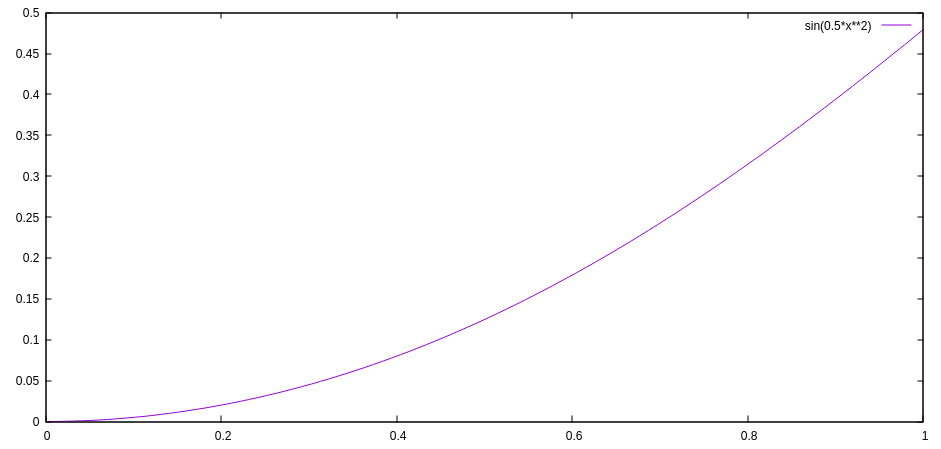
\includegraphics[scale=.666]{plot4.png}
    \subparagraph*{a:}
    Respectively, under, over, under, over
    \subparagraph*{b:}
    $L_n, M_n, T_n, R_n$
    \subparagraph*{c:}
    $T_5$
    
    \paragraph*{6:\\}
    $\int_{0}^{\pi} \! x \cos x \, \dx, n = 4$\\
    $M_4:\\ \Delta x = \frac{\pi}{4}$\\
    $\frac{\pi}{4} \cdot \sum\limits_{i=1}^{4} (\sin(\frac{1}{2} \cdot \frac{\pi}{4}))$
    $= \frac{\sqrt{2-\sqrt{2}}\cdot\pi}{2}$\\
    $\approx 1.20224$\\\\
    $S_4:\\$
    $x_0 = 0, x_1 = \pi/4, x_2 = \pi/2, x_3 = 3\pi/4, x_4 = \pi$\\
    $\frac{\frac{\pi}{4}}{3} [\sin(0) + 4\sin(\frac{\pi}{4}) + 2\sin(\frac{\pi}{2}) + 4\sin(\frac{3\pi}{4}) + \sin(\pi)]$

    \section{5.10:}
    $\int_{1}^{\infty} \! \frac{1}{x^p}\,\dx$ is convergent if $p > 1$ and divergent if $p \leq 1$
    \paragraph{1:\\}
    \subparagraph{a:} Goes to infinity
    \subparagraph{b:} Vertical asymptope
    \subparagraph{c:} Vertical asymptope
    \subparagraph{d:} Negative infinity
    \paragraph{2:\\}
    (c), infinity
    \paragraph{3:\\}
    Pretty much $0.5$. 
    \paragraph{5:\\}
    Convergent. \\
    $\int_{3}^{\infty} \! \frac{1}{(x-2)^{\frac{3}{2}}}\,\dx$\\
    $\lim_{t\to\infty} \int_{3}^{t} \! \frac{1}{(x-2)^{\frac{3}{2}}}\,\dx$\\
    $\int\!\frac{1}{(x-2)^{\frac{3}{2}}}\,\dx$
    $= \frac{-2}{\sqrt{x-2}}$\\
    $=-2$\\
    \paragraph{7:\\}
    divergent
    \paragraph{11:\\}
    divergent
    \paragraph{13:\\}
    convergent, $=0$

    \paragraph{15:\\}
    divergent
    \paragraph{19:\\}
    divergent
    \paragraph{21:\\}
    convergent, $=\frac{\pi}{9}$
    \paragraph{25:\\}
    divergent
    \paragraph{26:\\}
    convergent, $=2$\\
    \paragraph{33:\\}
    convergent, $=\frac{8\cdot(3\cdot\ln{2}-1}{9}$
      % \paragraph*{5.9:} 1, 2, 4, 6, 9, 12, 16, 18, 19
    % \paragraph*{5.10:} 1, 2, 3, 5, 7, 11, 13, 15, 19, 21, 25, 26, 33, 37, 39, 45

\thispagestyle{fancy}

\end{document}

